%!TEX root = MemoireZelliges.tex

\chapter{Présentation des échantillons}
%======================================================================

Les cinq échantillons que j'ai étudiés pendant mon stage au CRPAA 
proviennent du \PaM, daté du \siecle{xvii} et situé dans Meknès, 
la Versailles du Maroc.

\section{Meknès, capitale de Moulay Ismaïl}
%----------------------------------------------------------------------

Meknès (\fref{fig:maroc}) est la Cité Impériale de Moulay Ismaïl, 
second sultan de la dynastie alaouite. Lorsqu'il monta sur le trône 
en 1672, il en fit sa capitale et y entreprit des travaux de grande 
envergure pour en faire l'égal de Versailles qu'il admirait. 
L'ancienne casbah mérinide fut rasée pour faire place à des monuments 
grandioses, palais, mosquées, casbah, greniers et jardins, à l'abri 
derrière plus de quarante kilomètres d'un triple rempart de pierre. 
La mort de Moulay Ismaïl en 1727 et les guerres de succession qui 
en découlèrent mirent un terme prématuré aux travaux. Il perdit 
rapidement son rôle de résidence royale et Fès redevint la capitale 
du pays. Trois cents ans plus tard, Meknès est toujours une ville 
majestueuse, elle a été classée en décembre 1996 au Patrimoine 
Universel de l'Humanité par la commission intergouvernementale de 
l'U.N.E.S.C.O.

\begin{figure}[htb]
  \includegraphics[width=0.66\textwidth]{maroc}
  \caption{Meknès, Maroc.}
  \label{fig:maroc}
\end{figure}

\section{Le \PaM}
%----------------------------------------------------------------------

Ce palais, aussi appelé \emph{Heri el-Mensour}, porte le nom de son 
constructeur, un chrétien converti à l'Islam. Il est situé au sud de 
la qasba (\fref{fig:meknes}). Bien que délabré aujourd'hui, cet 
édifice est encore impressionnant \autocite{Barrucand_1976}.

\begin{figure}[htb]
  \includegraphics[width=0.95\textwidth]{meknes}
  \caption{Localisation du \PaM dans Meknès.}
  \label{fig:meknes}
\end{figure}

La première description du \PaM a été faite par Al-Zayyani : 
\frquote{Ismaïl avait encore fait construire dans la qasba un palais 
appelé al-Mansour : ce palais renfermait vingt coupoles, et chacune 
de ces coupoles avait une tour d'où l'on dominait le panorama formé 
par les plaines et les montagnes de Méquinez. {\dots} Il plafonne à 
plus de \num{100}~coudées : \num{50}~coudées pour le rez-de-chaussée 
et \num{50}~coudées pour le reste. Ce palais est composé de vingt 
salons, éclairés chacun par une fenêtre au milieu. Les fenêtres 
étaient grillagées et permettaient aux habitants d'avoir une vue des 
plaines de Meknès située toute entière entre deux montagnes. Les 
salons avaient un plafond en bois coloré et une toiture de tuiles 
vertes. Quatre de ces salons étaient longs de \num{70}~empans, les 
autres étant de \num{40}~empans de longs chacun {\dots}}
\autocite{Barrucand_1976}.

Il est surprenant de constater que ce bâtiment apparemment 
assez extraordinaire ne figure guère dans les récits des 
esclaves, ambassadeurs ou religieux qui ont décrit le Meknès du
\siecle{xvii}. Seul Joseph de Léon semble le connaître. Selon lui, 
les concubines tombées en disgrâce du sultan étaient reléguées dans ce 
palais périphérique. En fait, ce bâtiment aurait peut-être pu n'être 
construit qu'à l’extrême fin du règne de Moulay Ismaïl.

\begin{figure}[htb]
  \includegraphics[width=0.66\textwidth]{palais}
  \caption{Palais al-Mansour, Meknès, \scl{xvii}. Plan d'ensemble 
           \autocite{Barrucand_1976}}
  \label{fig:palais}
\end{figure}

Le \emph{Heri el-Mensour} (\fref{fig:palais}) est une bâtisse de forme 
parallélépipédique dont la façade est longue de \SI{79}{\m} et dont la 
profondeur est de \SI{92}{\m}. Un bâtiment annexe qui abrite notamment 
\emph{Bab Heri el-Mensour} prolonge la façade de \SI{31}{\m} vers le 
sud-est.

La profondeur de cette construction mitoyenne est de \SI{12}{\m}. 
La hauteur du \emph{heri} varie entre 
\SIrange[range-phrase=\ et\ ]{12}{14}{\m} (\autocite{Barrucand_1976}.

Ce bâtiment comporte un rez-de-chaussée et un étage. Les témoignages 
littéraires et les constatations archéologiques ont permit de mettre 
en évidence les fonctions utilitaires et subalternes du 
rez-de-chaussée. L'étage supérieur (\fref{fig:etage}) semble avoir eu 
des fonctions nettement plus nobles. Il n'est accessible que par un 
escalier moderne remplaçant la rampe d'origine et situé dans l'angle 
nord-est de l'édifice. Il est dans un état de délabrement avancé. Les 
constructions se distribuent sur les deux longs côtés d'une grande 
cour centrale mesurant \SI{76.80}m sur \SI{25.45}{\m} Elles sont 
groupées dans une double rangée sur le côté sud et dans une triple 
rangée sur le côté nord \autocite{Barrucand_1976}.


\begin{figure}[htb]
  \includegraphics[width=0.8\textwidth]{palais_etage}
  \caption{Palais al-Mansour, Meknès, \scl{xvii}. 
           Plan de l'étage. En rouge : point de prélèvement 
           (réalisation : A.~\bsc{Benmlih} et M.~\bsc{Haddad})}
  \label{fig:etage}
\end{figure}

L'ordonnance de la cour étonne par son irrégularité. Il semble s'être 
agit d'une grande cour d'honneur mais il n'y a plus de restes d'un 
éventuel portique et les nombreuses ouvertures dans les flancs nord 
et sud, disposées sans aucun souci d'axialité, étaient surmontées 
indifféremment de linteaux plats ou d'arcs brisés outrepassés. On 
reconnaît certaines constructions à deux étages percées de fenêtres. 
Si cet étage avait réellement servi de palais à Moulay Ismaïl ou 
même seulement à ses concubines disgraciées, il aurait comporté 
\emph{hammams}, fours, et, bien entendu, salle de prière. 
Des investigations plus poussées seraient nécessaires pour cerner 
de plus près les destinations et l'aménagement de cet étage 
\autocite{Barrucand_1976}.

\section{Les échantillons}
%----------------------------------------------------------------------

Les cinq échantillons de zelliges (planche~1) ont été prélevés sur 
le sol d'une salle située à l'étage du \PaM, au sud de la grande cour 
centrale (\fref{fig:etage}). Ce sont des pièces de céramique glaçurée 
de forme parallélépipédique. Chacune comporte une glaçure monochrome. 
L'échantillon référencé \bdx{6528} présente une glaçure verte, le 
\bdx{6529}, une glaçure bleu-vert, le \bdx{6530}, une glaçure noire, 
le \bdx{6531}, une glaçure miel et le \bdx{6532}, une glaçure blanche. 
Il s'agit là des cinq couleurs de base de l'art des zelliges.

Le \bdx{6529} est sensiblement plus gros et plus épais que les autres 
et, contrairement à eux, n'est pas chanfreiné. Il s'agit probablement 
d'un carreau entourant les motifs de zelliges.


[Planche des échantillons]


\chapter{Méthodologie et expérimentation}
%======================================================================

\section{Mémorisation des échantillons}
%----------------------------------------------------------------------

La première étape, avant toute intervention sur l'échantillon, est sa 
mémorisation.

Dès son arrivée au laboratoire, l'échantillon est photographié, 
scanné, dessiné. On note également ses dimensions et sa masse.

Ces préliminaires sont indispensables pour conserver une image de 
l'objet dans son état initial.

Les prises de vue ont été réalisées à l'aide d'un boîtier 
photographique \num{24x36} muni d'un objectif macro Nikon. 
L'éclairage de l'objet est assuré par des lampes tungstène 
\SI{75}{\W}. Le film photographique utilisé a une sensibilité 
de \SI{64}{ASA}.

\section[SAO et \CHRO]
        {Étude de la couleur : \SAO et \CHRO}
%----------------------------------------------------------------------

\subsection[SAO]
           {Détermination des ions chromogènes : \SAO}
%~~~~~~~~~~~~~~~~~~~~~~~~~~~~~~~~~~~~~~~~~~~~~~~~~~~~~~~~~~~~~~~~~~~~~~
La couleur résulte de l'interaction entre lumière et matière. Dans le 
cas des verres silicatés, elle est due à l'absorption spécifique du 
rayonnement lumineux par des cations de métaux de transition ou des 
terres rares présents à l'état d'impuretés dans la structure du verre 
\autocite{Lajarte_1979}.

En \SAO en mode réflexion diffuse, l'échantillon est bombardé 
par un rayonnement électromagnétique monochromatique. La mesure du 
rayonnement réfléchi (détecteur : photomultiplicateur) par la surface 
analysée permet de déterminer le spectre d'absorption. Celui-ci peut 
présenter des bandes d'absorption caractéristiques des ions 
chromogènes responsables de la couleur.

L'appareillage utilisé est un spectrophotomètre UV-visible 
double-faisceau (CARY1, Varian). La gamme spectrale balayée s'étend 
de \SIrange[range-phrase=\ à\ ]{190}{900}{\nm}.
La source du rayonnement est une lampe tungstène dans l'infrarouge 
et le visible, une lampe au deutérium prend le relais à \SI{310}{\nm}. 
On utilise une cellule de polytétrafluoroéthylène (PTFE) pour calibrer 
le système et comme blanc de référence.

Pour effectuer des mesures sur des zones de faibles dimensions, 
nous avons utilisé un montage couplant un microscope optique au 
spectrophotomètre. L'objet à étudier est placé sur la platine du 
microscope, l'éclairage, de type halogène, est assuré par des fibres 
optiques Intralux~5000. La gamme spectrale balayée est alors comprise 
entre \SIrange[range-phrase=\ et\ ]{380}{750}{\nm}. La lumière 
réfléchie par l'échantillon et reçue par l'objectif du microscope est 
dirigée vers le détecteur du spectrophotomètre par l'intermédiaire 
d'une autre fibre optique. Une étude méthodologique a permis de 
montrer que les résultats obtenus par cette méthode ne diffèrent pas 
sensiblement de ceux obtenus avec le spectrophotomètre seul (Baras, 
2000, DESS).

Cette méthode est non-destructive et ne nécessite aucun prélèvement de 
matière. Les mesures sont effectuées directement sur l'échantillon.

Les spectres d'\AO présentés sont ceux de l'objet composite (glaçure + 
terre cuite). Ils n'ont pas été corrigés de la contribution du support 
céramique lorsque la glaçure est transparente.

\subsection[Chromamétrie]{Mesure physique de la couleur : \CHRO}
%~~~~~~~~~~~~~~~~~~~~~~~~~~~~~~~~~~~~~~~~~~~~~~~~~~~~~~~~~~~~~~~~~~~~~~
La définition d'une couleur est particulièrement subjective et dépend 
de la sensibilité spectrale de l'{\oe}il, de la nature de la lumière 
incidente, de l'état de surface de l'objet, mais aussi de la culture 
et de l'éducation de l'observateur (les papous, par exemple, n'ont pas 
de terme pour désigner le jaune (\textit{Pour la Science}, hors-série 
avril 2000)).

La \CHRO permet de définir les couleurs par leurs
coordonnées chromatiques. Elle repose sur le fait que toute couleur
peut être définie comme la superposition de trois couleurs dites
\frquote{primaires} : le rouge, le vert et le bleu.

Conformément aux conventions mises en place par la \emph{Commission 
Internationale de l'Éclairage}, les modes de représentations 
graphiques choisis correspondent aux systèmes \Yxy (CIE~1931) 
(\fref{fig:Yxy}) et \Lab (CIE~1976) (\fref{fig:Lab}).

Le système \Lab peut être déduit du système \Yxy par transformation 
non linéaire :
\begin{align}
  \CIEL & =\ 116\ \left(\frac{Y}{\Yn}\right)^{1/3} - 16 \\
%
  \CIEa & =\ 500\ \left[%
      \left(\frac{X}{\Xn}\right)^{1/3} - %
      \left(\frac{Y}{\Yn}\right)^{1/3}%
    \right] \\
%
  \CIEb & =\ 200\ \left[%
      \left(\frac{Y}{\Yn}\right)^{1/3} - %
      \left(\frac{Z}{\Zn}\right)^{1/3}%
    \right]
\end{align}

\noindent
avec\quad $ \left\{\begin{lgathered}%[t]
  \begin{pmatrix}\Xn\\\Yn\\\Zn\end{pmatrix}\ 
  \text{coordonnées du point de référence}\\
  %
  \displaystyle\frac{X}{\Xn}\text{, }
  \displaystyle\frac{X}{\Xn}\text{, }
  \displaystyle\frac{X}{\Xn}\ >\ 0,008856
\end{lgathered}\right.$

\bigskip

Les paramètres \CIEY et \CIEL représentent la réflectance, c'est 
à dire la fraction de l'intensité de lumière réfléchie par l'aire 
examinée. Les paramètres \CIEx et \CIEy indiquent respectivement 
la proportion de photons rouges et verts dans la lumière réfléchie. 
\CIEz, représentant la composante bleu, est relié à \CIEx et \CIEy 
par :
\begin{equation}
  \CIEx + \CIEy + \CIEz = 1
\end{equation}

\CIEa représente la composante chromatique rouge-vert et \CIEb la 
composante bleu-jaune. L'espace \Lab, obtenu par transformation non 
linéaire de l'espace \Yxy, est particulièrement utilisé car c'est 
un espace uniforme : la distance de deux points de couleur est 
proportionnelle aux différences perçues par l'{\oe}il entre les 
réalisations colorées. Il est plus difficile de faire une corrélation 
entre écart chromatique et écart visuel dans le système \Yxy. 
En revanche, il permet l'obtention aisée de la longueur d'onde 
dominante \WLd du rayonnement, c'est à dire la longueur d'onde de la 
radiation spectrale qui, mélangée à une quantité appropriée de lumière 
blanche donne une égalisation colorimétrique de la couleur donnée, et 
de la pureté d'excitation représentant la quantité de lumière saturée 
caractérisée par \WLd dans le rayonnement.

\begin{figure}[htb]
  \begin{minipage}[b]{0.40\textwidth}%
    \centerfloat
    \begin{tikzpicture}
      \node [anchor=south west, inner sep=0] (image) at ( 0.00, 0.00) 
            {\includegraphics[width=\textwidth]{chroma_Yxy}} ;
      \begin{scope}[x={(image.south east)}, y={(image.north west)}]
        % \draw [step=0.05, help lines, white] (0, 0) grid (1, 1) ;

        \node [above] at ( 0.00, 1.00) {\CIEyb} ;
        \node [above right] at ( 1.00, 0.00) {\CIExb} ;
      \end{scope}
    \end{tikzpicture}
    \subcaption{Système \Yxy (CIE~1931)\label{fig:Yxy}}
  \end{minipage}%
  \hfill%
  \begin{minipage}[b]{0.45\textwidth}%
    \centerfloat
    \begin{tikzpicture}
      \node [anchor=south west, inner sep=0] (image) at ( 0.00, 0.00) 
            {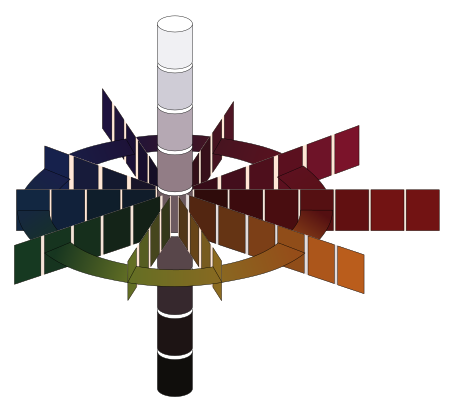
\includegraphics[width=\textwidth]{chroma_Lab}} ;
      \begin{scope}[x={(image.south east)}, y={(image.north west)}]
        % \draw [step=0.05, help lines, red] (0, 0) grid (1, 1) ;

        \node at ( 0.30, 0.90) {\CIELb} ;
        \node at ( 0.52, 0.25) {\CIEbb} ;
        \node at ( 0.83, 0.67) {\CIEab} ;
      \end{scope}
    \end{tikzpicture}
    \subcaption{Système \Lab (CIE~1976)\label{fig:Lab}}
  \end{minipage}%
  \caption[Systèmes colorimétriques \trichros]
          {Systèmes colorimétriques \trichros (\emph{Pour la science}, 
           hors série avril 2000)}
  \label{fig:colorimetrie}
\end{figure}


\definecolor{c0000ff}{RGB}{0,0,255}


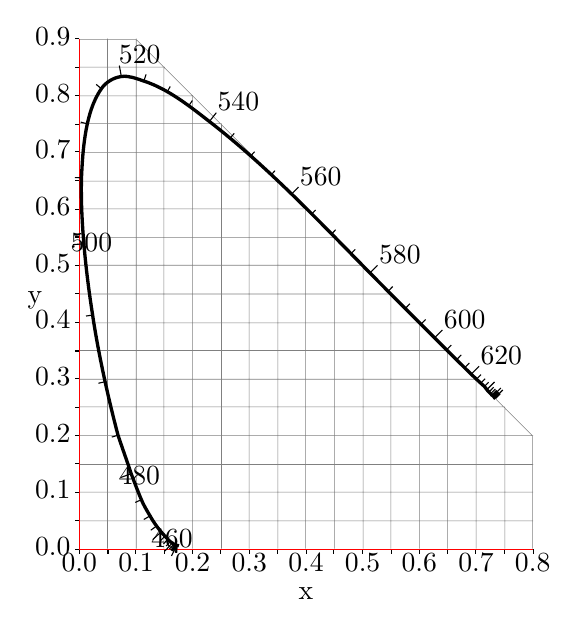
\begin{tikzpicture}[
  y=0.4pt, x=0.4pt, 
  yscale=-1, 
  inner sep=0pt, outer sep=0pt,
  % line width=0.8pt,
]
  \begin{scope}% g3528
    % path3530
    \draw [gray, very thin] 
          (74.6938,485.5000) -- (74.6938,24.7000) 
          (100.6939,485.5000) -- (100.6939,24.7000)
          (125.6939,485.5000) -- (125.6939,50.3000)
          (151.6939,485.5000) -- (151.6939,75.9000)
          (177.6939,485.5000) -- (177.6939,101.5000)
          (202.6939,485.5000) -- (202.6939,127.1000)
          (228.6939,485.5000) -- (228.6939,152.7000)
          (253.6939,485.5000) -- (253.6939,178.3000)
          (279.6939,485.5000) -- (279.6939,203.9000)
          (305.6939,485.5000) -- (305.6939,229.5000)
          (330.6939,485.5000) -- (330.6939,255.1000)
          (356.6939,485.5000) -- (356.6939,280.7000)
          (381.6939,485.5000) -- (381.6939,306.3000)
          (407.6939,485.5000) -- (407.6939,331.9000)
          (433.6939,485.5000) -- (433.6939,357.5000)
          (458.6939,485.5000) -- (458.6939,383.1000)
          (49.6938,460.5000) -- (459.2939,460.5000)
          (49.6938,434.5000) -- (459.2939,434.5000)
          (49.6938,409.5000) -- (459.2939,409.5000)
          (49.6938,383.5000) -- (459.2939,383.5000)
          (49.6938,357.5000) -- (433.6939,357.5000)
          (49.6938,332.5000) -- (408.0939,332.5000)
          (49.6938,306.5000) -- (382.4939,306.5000)
          (49.6938,281.5000) -- (356.8939,281.5000)
          (49.6938,255.5000) -- (331.2939,255.5000)
          (49.6938,229.5000) -- (305.6939,229.5000)
          (49.6938,204.5000) -- (280.0939,204.5000)
          (49.6938,178.5000) -- (254.4939,178.5000)
          (49.6938,153.5000) -- (228.8939,153.5000)
          (49.6938,127.5000) -- (203.2939,127.5000)
          (49.6938,101.5000) -- (177.6939,101.5000)
          (49.6938,76.5000) -- (152.0939,76.5000)
          (49.6938,50.5000) -- (126.4939,50.5000)
          (49.6938,25.5000) -- (100.8939,25.5000)
          (100.6939,25.5000) -- (458.6939,383.5000) ; 
  \end{scope}

  % Axes
  \begin{scope}
    \draw []
          (49.1938,25.0000) -- (49.1938,486.0000) --
          (459.1939,486.0000)
          (49.1938,486.0000) -- (49.1938,490.0000)
          (75.1938,486.0000) -- (75.1938,490.0000)
          (100.1939,486.0000) -- (100.1939,490.0000)
          (126.1939,486.0000) -- (126.1939,490.0000)
          (151.1939,486.0000) -- (151.1939,490.0000)
          (177.1939,486.0000) -- (177.1939,490.0000)
          (203.1939,486.0000) -- (203.1939,490.0000)
          (228.1939,486.0000) -- (228.1939,490.0000)
          (254.1939,486.0000) -- (254.1939,490.0000)
          (279.1939,486.0000) -- (279.1939,490.0000)
          (305.1939,486.0000) -- (305.1939,490.0000)
          (331.1939,486.0000) -- (331.1939,490.0000)
          (356.1939,486.0000) -- (356.1939,490.0000)
          (382.1939,486.0000) -- (382.1939,490.0000)
          (407.1939,486.0000) -- (407.1939,490.0000)
          (433.1939,486.0000) -- (433.1939,490.0000)
          (459.1939,486.0000) -- (459.1939,490.0000) ;

    \draw []
          (49.1938,486.0000) -- (45.1938,486.0000)
          (49.1938,460.0000) -- (45.1938,460.0000)
          (49.1938,435.0000) -- (45.1938,435.0000)
          (49.1938,409.0000) -- (45.1938,409.0000)
          (49.1938,383.0000) -- (45.1938,383.0000)
          (49.1938,358.0000) -- (45.1938,358.0000)
          (49.1938,332.0000) -- (45.1938,332.0000)
          (49.1938,307.0000) -- (45.1938,307.0000)
          (49.1938,281.0000) -- (45.1938,281.0000)
          (49.1938,255.0000) -- (45.1938,255.0000)
          (49.1938,230.0000) -- (45.1938,230.0000)
          (49.1938,204.0000) -- (45.1938,204.0000)
          (49.1938,179.0000) -- (45.1938,179.0000)
          (49.1938,153.0000) -- (45.1938,153.0000)
          (49.1938,127.0000) -- (45.1938,127.0000)
          (49.1938,102.0000) -- (45.1938,102.0000)
          (49.1938, 76.0000) -- (45.1938, 76.0000)
          (49.1938, 51.0000) -- (45.1938, 51.0000)
          (49.1938, 25.0000) -- (45.1938, 25.0000) ;

    \draw [shift={(45.1938, 490.0000)}, yscale=-1, red]
          ( 4.00, 4.00) -- ( 4.00, 465.00) ;
    \draw [shift={(45.1938, 490.0000)}, yscale=-1, red]
          ( 4.00, 4.00) -- ( 414.0001, 4.00) ;
  \end{scope}

  \begin{scope}
    \begin{scope}
      \begin{scope}[every node/.style={above}]
        \fill (49.193848,505.79999) node {0.0};
        \fill (100.39384,505.79999) node {0.1};
        \fill (151.59384,505.79999) node {0.2};
        \fill (202.79385,505.79999) node {0.3};
        \fill (253.99384,505.79999) node {0.4};
        \fill (305.19385,505.79999) node {0.5};
        \fill (356.39386,505.79999) node {0.6};
        \fill (407.59384,505.79999) node {0.7};
        \fill (458.79385,505.79999) node {0.8};
      \end{scope}
      \begin{scope}[every node/.style={above left}]
        \fill (41.193848,491.79999) node {0.0};
        \fill (41.193848,440.60001) node {0.1};
        \fill (41.193848,389.39999) node {0.2};
        \fill (41.193848,338.20001) node {0.3};
        \fill (41.193848,287) node {0.4};
        \fill (41.193848,235.8) node {0.5};
        \fill (41.193848,184.60001) node {0.6};
        \fill (41.193848,133.39999) node {0.7};
        \fill (41.193848,82.199997) node {0.8};
        \fill (41.193848,31) node {0.9};
      \end{scope}
    \end{scope}
    \begin{scope}
      \node at (253.99384,525.79999) {x};
      \node at (9.1938477,261.39999) {y};
    \end{scope}
  \end{scope}

  % Contour
  \begin{scope} [
    shift={(-10.80615,10.0)},
    very thick,
  ]
    \draw 
    (150.00,473.00) .. controls (147.00,473.00) and (145.00,471.00) ..
    (142.00,469.00) .. controls (135.00,462.00) and (129.00,455.00) ..
    (124.00,446.00) .. controls (121.00,441.00) and (118.00,436.00) ..
    (116.00,431.00) .. controls (113.00,424.00) and (110.00,416.00) ..
    (107.00,408.00) .. controls (103.00,396.00) and (99.00,385.00) ..
    (95.00,373.00) .. controls (86.00,339.00) and (77.00,298.00) ..
    (72.00,264.00) .. controls (66.00,226.00) and (61.00,179.00) ..
    (62.00,141.00) .. controls (63.00,118.00) and (65.00,81.00) ..
    (80.00,60.00) .. controls (84.00,54.00) and (91.00,50.00) ..
    (98.00,49.00) .. controls (105.00,48.00) and (112.00,51.00) ..
    (118.00,53.00) .. controls (140.00,60.00) and (160.00,76.00) ..
    (178.00,90.00) .. controls (236.00,135.00) and (287.00,191.00) ..
    (339.00,243.00) .. controls (360.00,264.00) and (380.00,284.00) ..
    (401.00,305.00) .. controls (409.00,313.00) and (417.00,321.00) ..
    (426.00,329.00) .. controls (428.00,332.00) and (430.00,334.00) ..
    (433.00,337.00) .. controls (434.00,337.00) and (434.00,338.00) ..
    (435.00,339.00) .. controls (435.00,339.00) and (436.00,340.00) ..
    (436.00,340.00) ;
  \end{scope}

  \begin{scope}% g3880
    % path3886
    \draw (137.5939,483.30) -- (137.1939,489.30)
          (137.2939,483.30) -- (135.9939,489.20)
          (136.9939,483.20) -- (132.4939,492.10)
          (136.3939,482.80) -- (132.9939,487.70)
          (135.6939,482.30) -- (131.8939,487.00)
          (134.6939,481.40) -- (130.6939,485.90)
          (133.3939,480.20) -- (126.6939,487.60)
          (131.6939,478.70) -- (127.6939,483.20)
          (129.3939,476.70) -- (125.3939,481.20)
          (126.4939,474.20) -- (122.3939,478.60)
          (122.8939,470.60) -- (115.4939,477.40)
          (118.5939,465.40) -- (113.7939,468.90)
          (112.6939,456.20) -- (107.4939,459.20)
          (105.2939,441.30) -- (99.7939,443.80)
          (95.8939,417.90) -- (86.4939,421.30)
          (84.3939,383.00) -- (78.5938,384.70)
          (72.3938,334.80) -- (66.4938,336.10)
          (61.1938,274.50) -- (55.2938,275.40)
          (53.3938,210.10) -- (43.3938,210.90)
          (51.1938,150.50) -- (45.1938,150.30)
          (56.2938,101.70) -- (50.4938,100.20)
          (69.0938,70.00) -- (64.4938,66.10)
          (87.1939,58.90) -- (85.3939,49.10)
          (107.6939,62.80) -- (109.5939,57.10)
          (128.3939,73.20) -- (131.3939,68.00)
          (147.9939,85.60) -- (151.3939,80.70)
          (166.7939,99.60) -- (172.9939,91.70)
          (185.2939,114.90) -- (189.1939,110.40)
          (203.5939,131.30) -- (207.5939,126.90)
          (221.8939,148.50) -- (225.9939,144.10)
          (240.1939,166.10) -- (247.1939,158.90)
          (258.4939,183.90) -- (262.6939,179.60)
          (276.5939,201.80) -- (280.7939,197.50)
          (294.2939,219.50) -- (298.4939,215.20)
          (311.5939,236.70) -- (318.6939,229.60)
          (328.0939,253.10) -- (332.2939,248.80)
          (343.6939,268.60) -- (347.8939,264.30)
          (357.8939,282.80) -- (362.0939,278.60)
          (370.1939,295.10) -- (377.2939,288.00)
          (381.0939,305.90) -- (385.2939,301.60)
          (390.0939,314.80) -- (394.2939,310.50)
          (397.3939,322.10) -- (401.5939,317.90)
          (403.2939,327.90) -- (410.3939,320.80)
          (407.8939,332.60) -- (412.0939,328.30)
          (411.6939,336.30) -- (415.8939,332.00)
          (414.7939,339.40) -- (418.9939,335.20)
          (417.2939,342.00) -- (424.3939,334.90)
          (419.3939,344.00) -- (423.5939,339.70)
          (420.8939,345.50) -- (425.0939,341.30)
          (422.0939,346.70) -- (426.2939,342.50)
          (422.8939,347.50) -- (429.9939,340.40)
          (423.4939,348.10) -- (427.6939,343.90)
          (423.9939,348.60) -- (428.1939,344.40)
          (424.3939,349.00) -- (428.5939,344.80)
          (424.6939,349.30) -- (431.7939,342.20)
          (424.9939,349.60) -- (429.1939,345.40)
          (425.1939,349.80) -- (429.3939,345.60)
          (425.2939,349.90) -- (429.4939,345.70) ;
  \end{scope}

  \begin{scope}[shift={(-10.80615,10.0)}]
    \node at (124.9,474.70001) [above right] {460} ;
    \node at (95.5,418) [above right] {480} ;
    \node at (52.200001,207.10001) [above right] {500} ;
    \node at (95.900002,37.099998) [above right] {520} ;
    \node at (185,80.099998) [above right] {540} ;
    \node at (259.39999,147.5) [above right] {560} ;
    \node at (330.89999,218.2) [above right] {580} ;
    \node at (389.5,276.60001) [above right] {600} ;
    \node at (422.5,309.39999) [above right] {620} ;
  \end{scope}
\end{tikzpicture}
%
\qquad%
%
\begin{tikzpicture}[
  line cap=round,
  % show background rectangle,
]

  % \pgfplotstableread{PaV.dat}{\pavdata}

  \begin{axis}[%
    xmin=0, xmax=0.8,
    ymin=0, ymax=0.9,
    width=8cm, height=9cm,
    axis lines*=left,
    tick align=outside,
    tick style={black, thin},
    ticklabel style={font=\small},
    minor tick num=3,
    xtick={0.0, 0.1, ..., 1.0},
    ytick={0.0, 0.1, ..., 1.0},
    minor tick={0.0, 0.05, ..., 1.0},
    % grid=both,
    xlabel=\CIExb, ylabel=\CIEyb,
    xlabel near ticks, ylabel near ticks,
    every axis x label/.style={
        at={(ticklabel* cs:1.0)},
        anchor=west,
    },
    every axis y label/.style={
        at={(ticklabel* cs:1.0)},
        anchor=south,
    },
    clip mode=individual,
  ]

    \begin{scope}
      \clip ( 0.0, 0.0) -- ( 0.0, 0.9) -- ( 0.1, 0.9) --
            ( 0.8, 0.2) -- ( 0.8, 0.0) -- cycle ;
      \draw [help lines, step=0.05] 
            ( 0.0, 0.0) grid ( 0.8, 0.9) ;
    \end{scope}
    \draw [help lines] 
          ( 0.0, 0.9) -- ( 0.1, 0.9) -- ( 0.8, 0.2) -- ( 0.8, 0.0) ;
    \draw ( 0.0, 0.9) -- ( 0.0, 0.0) -- ( 0.8, 0.0) ;

    \begin{scope}
      \addplot graphics [
        xmin=0.0036363842, xmax=0.7346900119, 
        ymin=0.0047740307, ymax=0.8340903145
      ]
        {pav} ;
    \end{scope}

    \begin{scope}[thick, line cap=round, line join=round]
      \addplot [thick, mark=none]
         table [x=x, y=y] 
               {\datadir/chro/CIE_espaces2D.dat} ;
      % \draw plot file {CIE_espaces2D.dat} -- cycle ;
    \end{scope}

%       \addplot [red, only marks, mark=|]
%          table [x=x, y=y] 
%                {
% x             y                   l
% 0.1439603960  0.0297029703        460
% 0.0912935070  0.1327020425        480
% 0.0081680280  0.5384230705        500
% 0.0743024248  0.8338030913        520
% 0.2296196726  0.7543290899        540
% 0.3731015439  0.6244508598        560
% 0.5124863668  0.4865907881        580
% 0.6270365998  0.3724911452        600
% 0.6915039730  0.3083422606        620
%                } ;
    % \begin{scope}
    %   \foreach \u/\v/\l in {
    %     0.1439603960/0.0297029703/460,
    %     0.0912935070/0.1327020425/480,
    %     0.0081680280/0.5384230705/500,
    %     0.0743024248/0.8338030913/520,
    %     0.2296196726/0.7543290899/540,
    %     0.3731015439/0.6244508598/560,
    %     0.5124863668/0.4865907881/580,
    %     0.6270365998/0.3724911452/600,
    %     0.6915039730/0.3083422606/620
    %   } {
    %     \node at (\u, \v) {\l} ;
    %   }
    % \end{scope}
  \end{axis}

  % \begin{scope}
  %   \foreach \x/\y/\l in {
  %     0.1439603960/0.0297029703/460,
  %     0.0912935070/0.1327020425/480,
  %     0.0081680280/0.5384230705/500,
  %     0.0743024248/0.8338030913/520,
  %     0.2296196726/0.7543290899/540,
  %     0.3731015439/0.6244508598/560,
  %     0.5124863668/0.4865907881/580,
  %     0.6270365998/0.3724911452/600,
  %     0.6915039730/0.3083422606/620
  %   }
  %     \node at (\x, \y) {\l} ;
  % \end{scope}



\end{tikzpicture}












Les mesures colorimétriques sont réalisées à partir des spectres 
d'\AO, par l'intermédiaire du module \frquote{Chromamétrie} intégré 
dans le système d'exploitation des données du spectrophotomètre. Ces 
mesures sont effectuées par rapport à l'illuminant standard D65, avec 
un angle solide d'observation de \ang{2} et dans la plage de longueur 
d'onde \SIrange{400}{700}{\nm}.

\section{Étude de la texture}
%----------------------------------------------------------------------

\subsection{Observation en lumière naturelle}
%~~~~~~~~~~~~~~~~~~~~~~~~~~~~~~~~~~~~~~~~~~~~~~~~~~~~~~~~~~~~~~~~~~~~~~
Préliminaire indispensable à toute étude, l'observation macroscopique 
permet d'examiner l'état de surface d'un échantillon, la cohésion de 
l'ensemble glaçure/terre cuite, de localiser d'éventuels défauts ou 
anomalies liées à la cuisson ou au processus d'altération. Cette étape 
est indispensable pour repérer les zones qui feront ultérieurement 
l'objet d'analyses approfondies.

Cet examen peut s'effectuer sur l'échantillon brut sans prélèvement 
de matière ou sur une coupe perpendiculaire à la surface.

On utilise une loupe binoculaire à effet de zoom Olympus SZH. 
L'échantillon est éclairé par des fibres optiques Intralux~5000. 
Des prises de vue peuvent être faites grâce à un boîtier 
photographique Olympus~SC35.

\subsection{Observation en \CL}
%~~~~~~~~~~~~~~~~~~~~~~~~~~~~~~~~~~~~~~~~~~~~~~~~~~~~~~~~~~~~~~~~~~~~~~
La \CL est l'émission de lumière induite par bombardement électronique 
d'un matériau isolant ou semi-conducteur.

Ce phénomène est dû à la présence, dans le réseau cristallin de 
certains minéraux, de défauts ponctuels tels que des lacunes (d'ion 
négatif), des atomes interstitiels ou de substitution (terres rares 
ou métaux de transition essentiellement), faisant apparaître des 
niveaux donneurs ou accepteurs d'électrons dans la bande interdite. 
Sous l'effet d'une excitation extérieure (ici un flux électronique), 
ces défauts peuvent capturer des électrons ou des trous. Leur 
désexcitation s'effectue par émission de photon dans le domaine 
du visible (\fref{fig:CL_principe}). On appelle ces défauts des 
\emph{centres luminogènes} ou \emph{centres colorés}.

La couleur de la luminescence dépend donc de défauts souvent 
caractéristiques d'un minéral et permet ainsi, avec l'appui de 
la \DX, l'identification des phases cristallines présentes dans 
un matériau (Bechtel, Platel, 2000).

L'observation en \CL donne également une idée de l'homogénéité de 
l'échantillon.

L'appareillage de \CL (\fref{fig:CL_app}) est constitué d'une chambre 
de type NUCLIDE maintenue sous vide primaire (\SI{5e-2}{\milli\bar}), 
d'un canon à électrons (cathode froide d'acier). La tension 
d'accélération est de l'ordre de \SI{10}{\kV} et l'intensité du 
courant se situe entre \SIrange[range-phrase=\ et\ ]{0.85}{0.95}{\mA}. 
Ce système est couplé à une loupe binoculaire et à une caméra 3CCD 
(Sony~DXC-930\,P) permettant l'enregistrement photographique.

\begin{figure}[htb]
  % \includegraphics[width=0.5\textwidth]{CL_principe}
  % \qquad
  \begin{tikzpicture}[remember picture]
    \CLpcp
  \end{tikzpicture}
  \begin{tikzpicture}[remember picture, overlay]
    \CLpcpL
  \end{tikzpicture}
  \caption[Principe de la \CL]
          {Principe de la \CL (d'après \cite{web_CL})}
  \label{fig:CL_principe}
\end{figure}
% (\url{http://loic.portelette.free.fr/aasaann.html}, avril 2000)

\begin{figure}
  % \includegraphics[width=0.5\textwidth]{CL_app}
  \begin{tikzpicture}[remember picture]
    \CLapp
  \end{tikzpicture}
  \begin{tikzpicture}[remember picture, overlay]
    \CLappL
  \end{tikzpicture}
  \caption{Appareillage de \CL}
  \label{fig:CL_app}
\end{figure}

L'analyse est généralement effectuée sur une lame, épaisse ou mince, 
taillée perpendiculairement à la surface glaçurée de l'échantillon 
et polie pour présenter la surface la plus plane possible.

Les lames sont réalisées à partir de prélèvement inclus dans une 
résine araldite. La découpe se fait à l'aide d'une scie à fil 
diamanté. On utilise pour le polissage des poudres de carbure 
de silicium (\SIrange[range-phrase=\ et\ ]{37}{9}{\um}) et des
suspensions diamantées de granulométrie progressive 
(\SIlist{6;3;1;0.1}{\um}).

\subsection{Observation en \MEB[ie]}
%~~~~~~~~~~~~~~~~~~~~~~~~~~~~~~~~~~~~~~~~~~~~~~~~~~~~~~~~~~~~~~~~~~~~~~
Le \MEB (MEB) est un instrument de visualisation permettant 
l'identification et la caractérisation de matériaux homogènes 
ou hétérogènes sur des surfaces allant du \si{\mm\squared} au
\si{\nm\squared} (grossissements de \texttimes\num{10} à 
\texttimes\num{300000}).

Il existe trois modes de formation des images en \MEB[ie] résultant 
de trois types d'interactions électrons-matière :

\begin{itemize}
  \item \uline{Imagerie en mode \emph{électrons secondaires}}\\
        Le faisceau peut provoquer l'arrachement d'électrons 
        périphériques des atomes de l'échantillon, ce sont les 
        électrons secondaires (\fref{fig:meb}). De faible énergie 
        (E=\SI{200}{\electronvolt}), ils proviennent de la surface 
        de l'échantillon et donnent une image de sa topographie. 
  \item \uline{Imagerie en mode \emph{\ERD}}\\ 
        Les \ERD (\fref{fig:meb}) proviennent de la diffusion 
        élastique ou quasi-élastique du faisceau incident. Ils ont 
        donc une énergie élevée, voisine de l'énergie incidente. 
        Les images obtenues présentent un contraste de composition : 
        en effet, le coefficient de rétrodiffusion est fonction de 
        la densité électronique, et donc du numéro atomique. 
        Autrement dit, les zones de l'échantillon correspondant aux 
        éléments les plus lourds, apparaîtront à l'écran plus claires, 
        plus \frquote{brillantes}. Les éléments légers correspondront 
        aux zones les plus noires de l'image.
  \item \uline{Imagerie par émission de \RX : \emph{\carto~X}}\\
        Le bombardement électronique primaire provoque aussi 
        l'émission de \RX caractéristiques de l'élément émetteur 
        (\fref{fig:meb}). Les cartes ainsi obtenues fournissent des 
        informations qualitatives sur la répartition des éléments 
        présents dans une couche superficielle.
\end{itemize}

\begin{figure}[htb]
  % \includegraphics[width=0.6\textwidth]{meb}
  \begin{tikzpicture}[remember picture]
    \MEBpoire
  \end{tikzpicture}
  \begin{tikzpicture}[remember picture, overlay]
    \MEBlegende
  \end{tikzpicture}
  \caption[Poire d'interaction électrons-matière]
          {Poire d'interaction électrons-matière 
           (d'après \cite{web_MEB})}
  \label{fig:meb}
\end{figure}

\section{Détermination des compositions élémentaires : \spectro de 
         \RX en dispersion d'énergie}
%----------------------------------------------------------------------

Pour déterminer les compositions élémentaires (majeurs et mineurs), 
on utilise l'analyse quantitative par \EDS (EDS).

L'échantillon à analyser est irradié par des électrons. L'interaction 
électrons-matière se traduit par différents phénomènes parmi lesquels 
l'émission de \RX. On obtient ainsi un spectre de raies se détachant 
du fond continu (rayonnement de freinage ou \emph{Bremsstrahlung}) 
caractéristique des éléments constitutifs de la matière. La méthode 
consiste à comparer l'intensité $I_A$ (en nombre de coups) 
correspondant à un élément $A$ de l'échantillon à celle produite 
dans les mêmes conditions par un échantillon témoin contenant $A$ 
en concentration connue. On a la relation suivante :

\begin{equation*}
  \frac{C_\text{A}}{C_\text{A témoin}} = 
                      k \frac{I_\text{A}}{I_\text{A témoin}}
\end{equation*}


avec%
\begin{description}
  \item [$C_\text{A}$] concentration en~A de l'échantillon
  \item [$C_\text{A témoin}$] concentration en~A du témoin
  \item [$I_\text{A}$] intensité du rayonnement correspondant à~A pour 
        l'échantillon
  \item [$I_\text{A témoin}$] intensité du rayonnement correspondant 
        à~A pour le témoin
  \item [$k$] facteur de correction ZAF
\end{description}

$k$ est un facteur correctif qui tient compte des différences de 
composition entre l'échantillon à analyser et le témoin. Il exprime 
les effets de matrice (on appelle matrice l'ensemble des éléments de 
l'échantillon en dehors de l'élément à analyser) tels que :

\begin{itemize}
  \item \uline{Effet de numéro atomique} : Pour une valeur incidente 
        égale, l'intensité électronique arrivant en un atome~A est 
        différente dans l'échantillon et dans le témoin, car les 
        électrons subissent des effets différents avant d'arriver en~A.
        La diminution d'intensité et d'énergie du faisceau dépend du 
        numéro atomique des éléments constituants ; il est nécessaire 
        d'en tenir compte par une correction dite \emph{correction de 
        numéro atomique} exprimée par le facteur~$k_\text{Z}$.
  \item \uline{Effet d'absorption} : L'absorption du rayonnement~X 
        caractéristique sur son trajet de sortie dépend également 
        de la composition. Le rapport des intensités après absorption
        dans l'échantillon et dans le témoin est différent du rapport 
        des intensités primaires émises ; on en tient compte par 
        la \emph{correction d'absorption} exprimée par le
        facteur~$k_\text{A}$.
  \item \uline{Effet de fluorescence} : Le rayonnement caractéristique 
        à mesurer peut également être produit par émission~X de 
        fluorescence, sous l'action de rayonnements~X caractéristiques 
        émis par des atomes B de la matrice plus lourds que les atomes 
        A. L'intensité mesurée est la somme des intensités primaire et 
        secondaire sortantes, après absorption. L'effet de 
        fluorescence étant différent dans l'échantillon et dans le 
        témoin, il faut en tenir compte par la \emph{correction de 
        fluorescence} exprimée par le facteur~$k_\text{F}$.
\end{itemize}

Au total, on a : $k = k_\text{Z} + k_\text{A} + k_\text{F}$

Le facteur k, nécessaire au calcul des concentrations, est calculé par 
une méthode itérative, dite \frquote{méthode ZAF}, avec, comme point 
de départ, $k=1$.

Pour que les comparaisons entre les intensités relatives à 
l'échantillon et celles relatives au témoin soient valables, les 
mesures doivent être effectuées dans les mêmes conditions de géométrie 
d'émission (même distance de travail, notamment) et de courant de 
sonde. Or, ce dernier est très variable. Pour remédier à ce dernier 
problème, on procède à une calibration par rapport à la raie $K_a$ 
du cobalt, dont le spectre a été enregistré en même temps que les 
spectres des témoins, et le système procède à des corrections pour 
se ramener aux conditions correspondant aux témoins.

On peut analyser les éléments à partir de $Z=5$ (bore), 
la résolution énergétique est de 
\SIrange[range-phrase=\ à\ ]{130}{150}{\electronvolt}, la limite de 
détection est de l'ordre de \SI{1000}{ppm}.

Les analyses quantitatives présentées dans ce mémoire sont données 
en pourcentages massiques d'oxyde normalisés à \SI{100}{\percent}. 
Ce sont des moyennes de trois à cinq mesures effectuées sur toute la 
longueur de la glaçure ou de la terre cuite, sur la zone d'analyse 
la plus grande possible, et en prenant garde d'éviter les bulles et 
cristaux non fondus. Ceci dans l'hypothèse où la \CL a permis de 
montrer l'homogénéité du matériau. L'oxygène est quantifié par 
différence.

On utilise un spectromètre de \RX en dispersion d'énergie couplé au 
\MEB (JEOL~850SM) et muni d'un détecteur semi-conducteur \ce{Si(Li)}.

\section[Diffraction de \RX]
        {Détermination des compositions \cristallos : \DX sur poudre}
%----------------------------------------------------------------------

L'état cristallin est caractérisé par une structure ordonnée et 
tripériodique. L'analyse par \DX sur poudre permet l'identification 
des phases cristallisées présentes dans un échantillon polycristallin.

Les \RX ont une longueur d'onde de l'ordre de la distance 
interatomique. Ils peuvent donc être diffractés par les plans 
interréticulaires du cristal selon la loi de Bragg (\fref{fig:DX_pcp} 
et équation~\ref{eqn:bragg}).


% \begin{equation*}
%   n \lambda = 2 d \cdot sin\theta
% \end{equation*}

% \bigskip

% \begin{minipage}{0.45\textwidth}
%   \begin{description}
%     \item [$d$] distance interréticulaire
%     \item [$\lambda$] longueur d'onde des \RX incidents
%     \item [$\theta$] angle d'incidence des \RX par rapport à la 
%           famille de plans réticulaires
%     \item [$n$] ordre de diffraction
%   \end{description}
% \end{minipage}%
% \hfill%
% \begin{minipage}{0.45\textwidth}
%   \begin{tikzpicture}[x=10mm, y=7mm]
%     \draw (-3.00, 0.00) -- ( 3.00, 0.00) ;
%     \draw (-3.00, 1.00) -- ( 3.00, 1.00) ;
%     \draw (-3.00,-1.00) -- ( 3.00,-1.00) ;

%     \begin{scope}[red, thick, >=Straight Barb]
%       \begin{scope}[postaction={decorate}, decoration={markings, 
%                     mark=at position 0.75 with 
%                     {\arrow[scale=1.67]{>};}}]
%         \draw [postaction={decorate}] ( 0.00, 0.00) -- ++ (  40:3) ;
%         \draw [postaction={decorate}] ( 0.00, 1.00) -- ++ (  40:3) ;
%       \end{scope}
%       \begin{scope}[postaction={decorate}, decoration={markings, 
%                     mark=at position 0.75 with 
%                     {\arrowreversed[scale=1.67]{>};}}]
%         \draw [postaction={decorate}] ( 0.00, 0.00) -- ++ ( 140:3) ;
%         \draw [postaction={decorate}] ( 0.00, 1.00) -- ++ ( 140:3) ;
%       \end{scope}
%     \end{scope}

%     \begin{scope}[shift={(3.25, 0.00)}]
%       \draw [<->] ( 0.00, 0.00) -- ( 0.00, 1.00) 
%             node [midway, right] {$d$} ;
%     \end{scope}

%     \draw ( 1.00, 0.00) arc (0:40:1) ;
%     \draw (-1.00, 0.00) arc (180:140:1) 
%           node [midway, left] {$\theta$} ;
%     \draw ( 1.00, 1.00) arc (0:40:1) ;
%     \draw (-1.00, 1.00) arc (180:140:1) ;
%   \end{tikzpicture}
% \end{minipage}


\begin{equation}\label{eqn:bragg}
  n\lambda = 2d\ sin\theta
\end{equation}

\bigskip  % \bigskip

\begin{figure}[h!]
  % \fbox{%
  \begin{minipage}{0.39\textwidth}
    \begin{itemize}  % \smaller
      \item [$d$ :] distance interréticulaire
      \item [$\lambda$ :] longueur d'onde des \RX incidents
      \item [$\theta$ :] angle d'incidence des \RX par rapport à la 
            famille de plans réticulaires
      \item [$n$ :] ordre de diffraction
    \end{itemize}
  \end{minipage}%
  % }%
  \hfill%
  % \fbox{%
  \begin{minipage}{0.56\textwidth}
    \centerfloat
    \begin{tikzpicture}
      \DXpcp
    \end{tikzpicture}
    \caption{Principe de \DX}
    \label{fig:DX_pcp}
  \end{minipage}%
  % }%
\end{figure}


  % \begin{figure}[htb]
  %   \begin{tikzpicture}
  %     \DXpcp
  %   \end{tikzpicture}
  %   \caption{Principe de \DX}
  %   \label{fig:DX_pcp}
  % \end{figure}


\bigskip

Dans la méthode de \DX sur poudre, le matériau à analyser est 
bombardé par un faisceau de \RX monochromatiques et parallèles, de 
longueur d'onde connue. L'échantillon, de quelques milligrammes, est 
étalé sous forme de poudre sur une lame de verre animée d'un mouvement 
de rotation uniforme autour d'un axe situé dans son plan (cercle 
goniométrique). De cette manière, chaque famille de plans réticulaires 
se présente sous toutes les orientations possibles par rapport au 
faisceau~X incident. Un détecteur mesure l'intensité du rayonnement~X 
diffracté. Il tourne autour du même axe que l'échantillon mais avec 
une vitesse double.

Le diffractogramme obtenu présente des raies, caractéristiques des 
phases cristallines présentes. L'identification s'effectue à l'aide 
d'un logiciel basé sur les fiches de référence ASTM (\emph{American 
Society for Testing and Materials}). La limite de détection est de 
\SI{2}{\percent}.

\begin{figure}[htb]
  % \includegraphics[width=0.6\textwidth]{DX}
  \begin{tikzpicture}
    \DXapp
  \end{tikzpicture}
  \caption{Appareillage de \DX}
  \label{fig:DX}
\end{figure}

L'équipement utilisé au laboratoire est un diffractomètre de 
poudre (\fref{fig:DX}) SIEMENS~D500. La source de \RX est une 
anticathode de cuivre ($\lambda=\SI{1.54}{\angstrom}$, 
$V=\SI{40}{\kV}$, $I=\SI{30}{\mA}$). Le domaine angulaire choisi 
pour l'étude s'étend de \ang{5} à \ang{60}.





